% ============================================================
%  ch4_System Design and Methodology.tex
%  Chapter 4: System Design and Methodology
%  Master's Thesis -- SQL MATCH_RECOGNIZE on Pandas DataFrames
% ============================================================
% Provide \mr if not already defined by the main document
\providecommand{\mr}{\texttt{MATCH\_RECOGNIZE}}
% !TEX root = Thesis.tex
\chapter{System Design and Methodology}
\label{chap:methodology}

This chapter describes how the engine turns a
\texttt{MATCH\_RECOGNIZE} query into an executable plan for a
Pandas DataFrame~\cite{monierashraf2025rowmatch}.  It also
explains the main design decisions.  The focus is the front end: the
stages that turn raw SQL into a validated execution configuration for
the implemented row-pattern subset~\cite{iso2016}.
Chapter~\ref{chap:implementation} continues with automata compilation,
execution, and optimization.

% ----------------------------------------------------------------
\section{Architecture Overview}
\label{sec:meth-overview}
% ----------------------------------------------------------------

The engine takes two inputs: an SQL query and a Pandas
DataFrame.  It returns a result DataFrame.  The work has five stages
(Figure~\ref{fig:system-architecture}).  \emph{Parsing} creates an
abstract syntax tree (AST).  \emph{Semantic validation} checks
references and supported clause combinations while the tree is built.
\emph{Logical-plan construction} resolves the execution configuration.
\emph{Pattern compilation} builds the automata.  Finally,
\emph{execution} combines the compiled pattern with the input and
builds the result.

The second stage is about meaning, not shape.  The grammar has already
proved the text well formed, so what remains is whether every
reference resolves and whether the requested clauses may be combined.
\texttt{AFTER MATCH SKIP TO LAST Z} over \texttt{PATTERN (A B)} parses
correctly, but \texttt{Z} is not a pattern variable.

These stages are design boundaries.  They do not require five separate
runtime objects: parsing and validation share one traversal, and the
logical plan is a group of resolved attributes.  The separation still
keeps errors close to their source and lets each boundary be tested
before matching begins.

\begin{figure}[htbp]
  \centering
  \begin{tikzpicture}[
    node distance=0.34cm,
    every node/.style={font=\small},
    input/.style={draw=gray!65, dashed, rounded corners=3pt,
                  line width=0.8pt, fill=gray!8, text width=2.45cm,
                  minimum height=0.95cm, align=center},
    phase/.style={draw=blue!55!black, rounded corners=3pt,
                  line width=0.9pt, fill=blue!6, text width=6.35cm,
                  minimum height=1.02cm, align=center, inner sep=5pt},
    execute/.style={phase, fill=blue!13},
    output/.style={draw=green!45!black, rounded corners=3pt,
                   line width=0.9pt, fill=green!9, text width=2.45cm,
                   minimum height=0.95cm, align=center},
    flow/.style={-{Stealth[length=2.3mm,width=1.6mm]},
                 line width=0.9pt, draw=blue!55!black},
    dataflow/.style={-{Stealth[length=2.3mm,width=1.6mm]},
                     line width=0.9pt, draw=gray!70!black}
  ]
    \node[phase] (parse)
      {\textbf{1. Parsing}\\[-1pt]
       \footnotesize SQL text $\longrightarrow$ abstract syntax tree};
    \node[phase, below=of parse] (validate)
      {\textbf{2. Semantic validation}\\[-1pt]
       \footnotesize check supported clauses and references};
    \node[phase, below=of validate] (plan)
      {\textbf{3. Logical-plan construction}\\[-1pt]
       \footnotesize resolve the execution configuration};
    \node[phase, below=of plan] (compile)
      {\textbf{4. Pattern compilation}\\[-1pt]
       \footnotesize pattern tokens $\longrightarrow$ NFA and complete DFA};
    \node[execute, below=of compile] (run)
      {\textbf{5. DataFrame execution}\\[-1pt]
       \footnotesize partition and order $\longrightarrow$ match\\[-1pt]
       \footnotesize evaluate measures $\longrightarrow$ assemble result};

    \node[input, left=0.68cm of parse] (sqlin)
      {\textbf{Input 1}\\SQL query};
    \node[input, left=0.68cm of run] (dfin)
      {\textbf{Input 2}\\Pandas DataFrame};
    \node[output, right=0.68cm of run] (dfout)
      {\textbf{Output}\\Result DataFrame};

    \draw[dataflow] (sqlin) -- (parse);
    \draw[flow] (parse) -- (validate);
    \draw[flow] (validate) -- (plan);
    \draw[flow] (plan) -- (compile);
    \draw[flow] (compile) -- (run);
    \draw[dataflow] (dfin) -- (run);
    \draw[dataflow] (run) -- (dfout);
  \end{tikzpicture}
  \caption{Five-stage architecture of the proposed engine.}
  \label{fig:system-architecture}
\end{figure}

The compiler converts the validated pattern into a non-deterministic
finite automaton (NFA) and then a complete deterministic finite
automaton (DFA)~\cite{HopcroftUllman}.  An NFA may be in several
states at once, so it represents alternation, optional parts, and
repetition directly.  A DFA has exactly one next state for each input,
so matching becomes a lookup instead of a search.  The conversion
therefore trades construction cost for a predictable scan.  If
complete construction exceeds a resource limit, compilation fails
explicitly; it never executes a partial automaton.  Chapter~\ref{chap:implementation}
explains compilation and DataFrame execution in detail.

% ................................
\subsection{Worked Pipeline Example}
\label{subsec:meth-worked-pipeline}
% ................................

Figure~\ref{fig:orders-pipeline} applies the architecture to the
\texttt{orders} example.  It carries both inputs, an SQL query and an
eight-row DataFrame, and traces them through the stages of
Figure~\ref{fig:system-architecture}.
Chapter~\ref{chap:evaluation} reuses the same example for the
usability comparison.

\begin{figure}[htbp]
  \centering
  \begin{tikzpicture}[
    node distance=0.26cm,
    every node/.style={font=\small},
    queryinput/.style={draw=gray!65, rounded corners=3pt,
                       line width=0.8pt, fill=gray!5,
                       align=left, inner sep=5pt},
    examplephase/.style={draw=blue!55!black, rounded corners=3pt,
                         line width=0.9pt, fill=blue!5,
                         text width=7.55cm, minimum height=1.02cm,
                         align=center, inner sep=5pt},
    examplecompile/.style={examplephase, minimum height=2.55cm},
    examplerun/.style={examplephase, fill=blue!10,
                       text width=2.65cm, minimum height=3.25cm},
    inputtable/.style={draw=gray!65, rounded corners=3pt,
                       line width=0.8pt, fill=gray!5,
                       align=center, inner sep=3pt},
    resulttable/.style={draw=green!45!black, rounded corners=3pt,
                        line width=0.9pt, fill=green!7,
                        align=center, inner sep=3pt},
    statepoint/.style={circle, draw=blue!55!black, line width=0.8pt,
                       fill=white, minimum size=0.54cm, inner sep=1pt,
                       font=\scriptsize},
    acceptpoint/.style={statepoint, double, double distance=1.1pt},
    exampleflow/.style={-{Stealth[length=2.3mm,width=1.6mm]},
                        line width=0.9pt, draw=blue!55!black},
    exampledata/.style={-{Stealth[length=2.3mm,width=1.6mm]},
                        line width=0.9pt, draw=gray!70!black}
  ]
    \node[examplephase] (exparse)
      {\textbf{1. Parsing}\\[-1pt]
       \footnotesize partition: \texttt{customer\_id};
       order: \texttt{order\_date}\\[-1pt]
       \footnotesize pattern: \texttt{A B C}; three measures; two definitions};
    \node[examplephase, below=of exparse] (exvalidate)
      {\textbf{2. Semantic validation}\\[-1pt]
       \footnotesize pattern-variable references are valid;
       $A\equiv\mathrm{true}$\\[-1pt]
       \footnotesize $B.\mathrm{price}<A.\mathrm{price}$;
       $C.\mathrm{price}<B.\mathrm{price}$};
    \node[examplephase, below=of exvalidate] (explan)
      {\textbf{3. Logical plan}\\[-1pt]
       \footnotesize \texttt{ONE ROW PER MATCH} (default)\\[-1pt]
       \footnotesize \texttt{SKIP PAST LAST ROW} (default)\\[-1pt]
       \footnotesize three measures $+$ partition key $\longrightarrow$ four columns};

    % Stage 4 shows the actual reachable DFA produced for PATTERN (A B C).
    \node[examplecompile, below=of explan] (excompile) {};
    \node[font=\small\bfseries]
      at ([yshift=0.97cm]excompile.center) {4. Pattern compilation};
    \node[font=\scriptsize]
      at ([yshift=0.64cm]excompile.center)
      {NFA (10 states) $\longrightarrow$ subset construction
       $\longrightarrow$ guarded DFA};
    \node[statepoint] (qzero)
      at ([xshift=-2.55cm,yshift=0.08cm]excompile.center) {$D_0$};
    \node[statepoint] (qone)
      at ([xshift=-0.85cm,yshift=0.08cm]excompile.center) {$D_1$};
    \node[statepoint] (qtwo)
      at ([xshift=0.85cm,yshift=0.08cm]excompile.center) {$D_2$};
    \node[acceptpoint] (qthree)
      at ([xshift=2.55cm,yshift=0.08cm]excompile.center) {$D_3$};
    \draw[exampleflow] ([xshift=-0.42cm]qzero.west) -- (qzero.west);
    \draw[exampleflow] (qzero) -- node[above,font=\scriptsize]{A} (qone);
    \draw[exampleflow] (qone) -- node[above,font=\scriptsize]{B} (qtwo);
    \draw[exampleflow] (qtwo) -- node[above,font=\scriptsize]{C} (qthree);
    \node[font=\scriptsize]
      at ([xshift=-2.55cm,yshift=-0.42cm]excompile.center) {$\{0,2,3\}$};
    \node[font=\scriptsize]
      at ([xshift=-0.85cm,yshift=-0.42cm]excompile.center) {$\{4,5\}$};
    \node[font=\scriptsize]
      at ([xshift=0.85cm,yshift=-0.42cm]excompile.center) {$\{6,7\}$};
    \node[font=\scriptsize]
      at ([xshift=2.55cm,yshift=-0.42cm]excompile.center) {$\{1,8,9\}$};
    \node[font=\scriptsize]
      at ([yshift=-0.77cm]excompile.center)
      {braces show the NFA states in each DFA state};
    \node[font=\scriptsize]
      at ([yshift=-1.02cm]excompile.center)
      {$D_3$ accepts; a missing transition rejects the candidate};

    % Stage 5 is deliberately compact; the adjacent tables carry the data.
    \node[examplerun, below=of excompile] (exrun)
      {\textbf{5. DataFrame}\\[-1pt]
       \textbf{execution}\\[3pt]
       \footnotesize partition $+$ order\\[-1pt]
       $\downarrow$\\[-1pt]
       \footnotesize DFA scan\\[-1pt]
       $\downarrow$\\[-1pt]
       \footnotesize measure evaluation\\[-1pt]
       $\downarrow$\\[-1pt]
       \footnotesize result assembly};

    \node[queryinput, above=0.30cm of exparse] (exquery)
      {\scriptsize
       \setlength{\tabcolsep}{0pt}
       \renewcommand{\arraystretch}{0.91}
       \begin{tabular}{@{}l@{}}
         \multicolumn{1}{c}{\normalsize\textbf{SQL query}} \\[2pt]
         \texttt{SELECT customer\_id, start\_date,} \\
         \texttt{\hspace*{2em}end\_date, bottom\_price} \\
         \texttt{FROM orders} \\
         \texttt{MATCH\_RECOGNIZE (} \\
         \texttt{\hspace*{1em}PARTITION BY customer\_id} \\
         \texttt{\hspace*{1em}ORDER BY order\_date} \\
         \texttt{\hspace*{1em}MEASURES} \\
         \texttt{\hspace*{2em}A.order\_date AS start\_date,} \\
         \texttt{\hspace*{2em}C.order\_date AS end\_date,} \\
         \texttt{\hspace*{2em}C.price AS bottom\_price} \\
         \texttt{\hspace*{1em}PATTERN (A B C)} \\
         \texttt{\hspace*{1em}DEFINE} \\
         \texttt{\hspace*{2em}B AS B.price < A.price,} \\
         \texttt{\hspace*{2em}C AS C.price < B.price} \\
         \texttt{);}
       \end{tabular}};
    \node[inputtable, left=0.18cm of exrun] (exdata)
      {\scriptsize
       \setlength{\tabcolsep}{1.5pt}
       \renewcommand{\arraystretch}{0.91}
       \arrayrulecolor{gray!55}
       \begin{tabular}{|l|c|r|}
         \hline
         \multicolumn{3}{|c|}{\cellcolor{gray!12}
           \textbf{Pandas DataFrame: \texttt{orders}}} \\
         \hline
         \rowcolor{gray!20}
         \texttt{customer\_id} & \texttt{order\_date} & \texttt{price} \\
         \hline
         cust\_1 & 2020-05-11 & 100 \\
         cust\_1 & 2020-05-12 & 200 \\
         cust\_2 & 2020-05-13 &   8 \\
         cust\_1 & 2020-05-14 & 100 \\
         cust\_2 & 2020-05-15 &   4 \\
         cust\_1 & 2020-05-16 &  50 \\
         cust\_1 & 2020-05-17 & 100 \\
         cust\_2 & 2020-05-18 &   6 \\
         \hline
       \end{tabular}};
    \node[resulttable, right=0.18cm of exrun] (exoutput)
      {\scriptsize
       \setlength{\tabcolsep}{1pt}
       \renewcommand{\arraystretch}{0.96}
       \arrayrulecolor{green!45!black}
       \begin{tabular}{|l|c|c|r|}
         \hline
         \multicolumn{4}{|c|}{\cellcolor{green!13}
           \textbf{Result DataFrame}} \\
         \hline
         \rowcolor{green!20}
         \shortstack{\texttt{customer}\\[-1pt]\texttt{\_id}} &
         \shortstack{\texttt{start}\\[-1pt]\texttt{\_date}} &
         \shortstack{\texttt{end}\\[-1pt]\texttt{\_date}} &
         \shortstack{\texttt{bottom}\\[-1pt]\texttt{\_price}} \\
         \hline
         cust\_1 & 2020-05-12 & 2020-05-16 & 50 \\
         \hline
       \end{tabular}};

    \draw[exampledata] (exquery) -- (exparse);
    \draw[exampleflow] (exparse) -- (exvalidate);
    \draw[exampleflow] (exvalidate) -- (explan);
    \draw[exampleflow] (explan) -- (excompile);
    \draw[exampleflow] (excompile) -- (exrun);
    \draw[exampledata] (exdata) -- (exrun);
    \draw[exampledata] (exrun) -- (exoutput);
  \end{tikzpicture}
  \caption{Worked \texttt{orders} pipeline.}
  \label{fig:orders-pipeline}
\end{figure}

The input table accounts for all eight rows.  Stage~4 shows the four
reachable DFA states produced for this pattern.  Each transition is
guarded by the predicate of its labeled variable.  During execution,
\texttt{cust\_1} satisfies $A\rightarrow B\rightarrow C$ with prices
$200>100>50$ and produces the output row.  The \texttt{cust\_2}
candidate fails at $C$ because $6<4$ is false.

The next three sections follow stages~1 to~3.
Section~\ref{sec:meth-compiler} covers parsing,
Section~\ref{sec:meth-semantic} semantic validation, and
Section~\ref{sec:meth-logical} logical-plan construction.
Chapter~\ref{chap:implementation} continues with Stage~4, pattern
compilation (Section~\ref{sec:meth-automata}), and Stage~5, DataFrame
execution (Section~\ref{sec:meth-pandas}).  The figure shows all five
because the two chapters form one pipeline.

% ----------------------------------------------------------------
\section{SQL Parsing}
\label{sec:meth-compiler}
% ----------------------------------------------------------------

Section~\ref{subsec:bg-clause-structure} described the clause
structure.  A \texttt{MATCH\_RECOGNIZE} query mixes ordinary SQL with
an extended row-pattern language, and the parser must handle both at
once.  Listing~\ref{lst:mr-full-syntax} gives the form the core path
accepts.

\begin{lstlisting}[float=htbp,
    language   = {},
    caption    = {Clause structure used by the supported
                  \texttt{MATCH\_RECOGNIZE} path},
    label      = {lst:mr-full-syntax},
    basicstyle = \ttfamily\footnotesize
]
SELECT <expression> [, ...]
FROM   <table>
MATCH_RECOGNIZE (
  [ PARTITION BY <column> [, ...] ]
  [ ORDER BY <column> [ASC|DESC] [NULLS FIRST|NULLS LAST] [, ...] ]
  [ MEASURES <expression> AS <alias> [, ...] ]
  [ ONE ROW PER MATCH
  | ALL ROWS PER MATCH
    [ SHOW EMPTY MATCHES
    | OMIT EMPTY MATCHES
    | WITH UNMATCHED ROWS ] ]
  [ AFTER MATCH SKIP
    { PAST LAST ROW
    | TO NEXT ROW
    | TO FIRST <variable>
    | TO LAST  <variable> } ]
  PATTERN ( <row_pattern> )
  [ SUBSET <subset_name> = ( <variable> [, ...] ) [, ...] ]
  [ DEFINE <variable> AS <condition> [, ...] ]
) [ AS <alias> ]
<rest>;
\end{lstlisting}

The core DataFrame path targets one \texttt{MATCH\_RECOGNIZE} clause
inside a top-level \texttt{SELECT}, with an optional outer
\texttt{ORDER~BY}.  A narrow separate path supports multiple
independent clauses over self-contained inline relations.  It is not a
general relational planner.  The \texttt{DEFINE} clause is optional,
and a pattern variable without a predicate is treated as always true.
Ordering keys support per-key \texttt{ASC}/\texttt{DESC} direction
and \texttt{NULLS FIRST}/\texttt{NULLS LAST}; omitted null placement
defaults to \texttt{NULLS LAST}.  A key may also be an expression over
the input columns, such as \texttt{ABS(ts)} or \texttt{price + ts}.
Conditional and subquery ordering keys, rewriting of \texttt{WITH}
clauses (CTEs), set-operation planning, and general nested subqueries
remain outside the supported path.

\paragraph{Choosing a parser.}
The requirement is a typed tree for both languages at once.  At the
time of design, none of the reviewed Python SQL libraries covered the
needed row-pattern syntax.
\texttt{sqlparse}~\cite{sqlparse_tool}
produces only a shallow token stream.
\texttt{sqlglot}~\cite{sqlglot_tool} and
\texttt{mo\_sql\_parsing}~\cite{mo_sql_parsing_tool} expose a typed AST
but omit constructs such as exclusions, anchors, \texttt{PERMUTE}, and
bounded quantifiers.  \texttt{pglast}~\cite{pglast_tool} cannot
parse \texttt{MATCH\_RECOGNIZE} at all.  Rather than extend one of
these, the engine reuses the community grammar for the Trino SQL
dialect written for ANTLR4, a parser generator that builds a parser
from a written grammar~\cite{antlr_trino_sql,Parr2013}.  Its
\texttt{patternRecognition} rule already covers all eight
sub-clauses.  ANTLR4 generates the lexer, parser, and traversal
scaffolding directly from that grammar, so no grammar changes were
needed.

Two ANTLR4 properties matter here.  Its adaptive $LL(*)$ prediction
examines more input when a decision needs it~\cite{parr2014adaptive}.
It also rewrites direct left-recursive expression rules internally.
This lets the Trino grammar keep its natural Boolean and arithmetic
structure.

Syntax errors go through a custom \emph{error listener} instead of
ANTLR's console default.  Each error carries a line, column, and source
snippet.  A hand-written recursive-descent parser would duplicate a
large SQL grammar.  Regular expressions also cannot model nested
pattern groups.

\paragraph{From parse tree to a typed AST.}
ANTLR4's parse tree is a \emph{concrete syntax tree}.  It contains the
full grammatical structure, including keywords and punctuation that
execution does not need.  The engine converts this tree to a simpler
abstract syntax tree (AST) using the \emph{Visitor}
pattern~\cite{robson2022designpatterns,Parr2013}.  This behavioral
design pattern separates an operation from the objects it acts on.
The same tree can then support different tasks, such as building an
AST or checking a query, without changing its node classes.

The \emph{client} starts the task.  The \emph{visitor interface}
defines an operation for each node type.  A \emph{concrete visitor}
provides the code for those operations.  The \emph{element interface}
allows a node to accept a visitor.  The \emph{concrete elements} are
the different node types in the tree, such as query and clause nodes.

The visitor passes itself to a node through an \texttt{accept}
method.  The node then calls the visitor operation for its own type.
The node type selects the operation, while the concrete visitor
determines what that operation does.  This two-part selection is
called \emph{double dispatch}.

Figure~\ref{fig:visitor-dispatch} shows this process as a pipeline using
\texttt{SELECT price FROM orders}.  The visitor records
\texttt{price} as the selected column and \texttt{orders} as the
source table.  The keywords guide parsing, but are not kept as
separate token nodes in the AST.  A different visitor could display
the same query parts instead.  The nodes stay the same; only the
visitor's task changes.

\begin{figure}[htbp]
  \centering
  \begin{tikzpicture}[
    every node/.style={font=\small},
    stage/.style={draw, rounded corners=3pt, line width=0.8pt,
                  align=center, text width=12.3cm, inner sep=5pt},
    input/.style={stage, draw=gray!70, fill=gray!8,
                  minimum height=1.2cm},
    element/.style={stage, draw=orange!70!black, fill=orange!8,
                    minimum height=4.2cm},
    visitor/.style={stage, draw=blue!55!black, fill=blue!7,
                    minimum height=5.4cm},
    result/.style={stage, draw=green!45!black, fill=green!8,
                   minimum height=3.0cm},
    treenode/.style={draw=orange!70!black, fill=white,
                     rounded corners=2pt, line width=0.6pt,
                     align=center, font=\footnotesize,
                     inner sep=4pt},
    keyword/.style={treenode, draw=gray!65, fill=gray!8,
                     text width=1.9cm},
    identifier/.style={treenode, fill=orange!12, text width=1.9cm},
    operation/.style={treenode, draw=blue!55!black,
                       text width=3.25cm, minimum height=1.4cm},
    astnode/.style={treenode, draw=green!45!black,
                     text width=3.8cm},
    flow/.style={-{Latex[length=2.2mm]}, line width=0.85pt,
                 draw=black!70}
  ]
    \node[input] (sql) {
      \textbf{1. Input SQL query}\\[3pt]
      \texttt{SELECT price FROM orders}};

    \node[element, below=0.7cm of sql] (element) {};
    \node[font=\small\bfseries]
      at ([yshift=1.72cm]element.center) {2. Simplified parse tree};
    \node[treenode, text width=1.4cm] (queryroot)
      at ([yshift=1.0cm]element.center) {Query};
    \node[treenode, text width=2.8cm] (selection)
      at ([xshift=-3.1cm,yshift=-0.05cm]element.center)
      {Selection clause};
    \node[treenode, text width=2.8cm] (source)
      at ([xshift=3.1cm,yshift=-0.05cm]element.center)
      {Source clause};
    \node[keyword] (selectkeyword)
      at ([xshift=-4.65cm,yshift=-1.25cm]element.center)
      {Keyword\\\texttt{SELECT}};
    \node[identifier] (columnname)
      at ([xshift=-1.55cm,yshift=-1.25cm]element.center)
      {Column\\\texttt{price}};
    \node[keyword] (fromkeyword)
      at ([xshift=1.55cm,yshift=-1.25cm]element.center)
      {Keyword\\\texttt{FROM}};
    \node[identifier] (tablename)
      at ([xshift=4.65cm,yshift=-1.25cm]element.center)
      {Table\\\texttt{orders}};
    \draw[draw=orange!70!black, line width=0.7pt]
      (queryroot.south) -- ++(0,-0.3cm) -| (selection.north);
    \draw[draw=orange!70!black, line width=0.7pt]
      (queryroot.south) -- ++(0,-0.3cm) -| (source.north);
    \draw[draw=orange!70!black, line width=0.7pt]
      (selection.south) -- ++(0,-0.3cm) -| (selectkeyword.north);
    \draw[draw=orange!70!black, line width=0.7pt]
      (selection.south) -- ++(0,-0.3cm) -| (columnname.north);
    \draw[draw=orange!70!black, line width=0.7pt]
      (source.south) -- ++(0,-0.3cm) -| (fromkeyword.north);
    \draw[draw=orange!70!black, line width=0.7pt]
      (source.south) -- ++(0,-0.3cm) -| (tablename.north);

    \node[visitor, below=0.7cm of element] (visitor) {};
    \node[font=\small\bfseries]
      at ([yshift=2.3cm]visitor.center) {3. Visitor processing};
    \node[font=\footnotesize, align=center, text width=11cm]
      at ([yshift=1.65cm]visitor.center)
      {The client starts the visit.  These steps repeat for each clause node.};
    \node[operation] (accept)
      at ([xshift=-4.15cm,yshift=0.55cm]visitor.center)
      {\textbf{a. Accept visitor}\\Node receives\\the visitor.};
    \node[operation] (dispatch)
      at ([yshift=0.55cm]visitor.center)
      {\textbf{b. Call operation}\\Node calls the\\visitor's operation.};
    \node[operation] (record)
      at ([xshift=4.15cm,yshift=0.55cm]visitor.center)
      {\textbf{c. Record details}\\Visitor keeps\\the needed details.};
    \draw[flow] (accept) -- (dispatch);
    \draw[flow] (dispatch) -- (record);
    \node[font=\footnotesize]
      at ([yshift=-0.65cm]visitor.center)
      {Examples of matching operations};
    \node[operation, text width=4.6cm, minimum height=1.1cm]
      at ([xshift=-3.1cm,yshift=-1.55cm]visitor.center)
      {\textbf{Selection operation}\\Record column: \texttt{price}};
    \node[operation, text width=4.6cm, minimum height=1.1cm]
      at ([xshift=3.1cm,yshift=-1.55cm]visitor.center)
      {\textbf{Source operation}\\Record table: \texttt{orders}};

    \node[result, below=0.7cm of visitor] (result) {};
    \node[font=\small\bfseries]
      at ([yshift=1.12cm]result.center) {4. Output AST: query structure};
    \node[astnode, text width=1.4cm] (astroot)
      at ([yshift=0.45cm]result.center) {Query};
    \node[astnode] (astcolumn)
      at ([xshift=-3.1cm,yshift=-0.65cm]result.center)
      {Selected column\\\texttt{price}};
    \node[astnode] (asttable)
      at ([xshift=3.1cm,yshift=-0.65cm]result.center)
      {Source table\\\texttt{orders}};
    \draw[draw=green!45!black, line width=0.7pt]
      (astroot.south) -- ++(0,-0.25cm) -| (astcolumn.north);
    \draw[draw=green!45!black, line width=0.7pt]
      (astroot.south) -- ++(0,-0.25cm) -| (asttable.north);

    \draw[flow] (sql) -- node[right, font=\footnotesize]
      {Parse the query} (element);
    \draw[flow] (element) -- node[right, font=\footnotesize]
      {Visit the tree} (visitor);
    \draw[flow] (visitor) -- node[right, font=\footnotesize]
      {Build the AST} (result);
  \end{tikzpicture}
  \caption[Visitor pipeline: from SQL to an AST]{Pipeline for
    \texttt{SELECT price FROM orders}.  Steps a and b show double
    dispatch: the node selects the operation, and the visitor supplies
    its behavior.  Keyword tokens are not kept as separate AST nodes.
    The output describes the query; it does not contain query results.}
  \label{fig:visitor-dispatch}
\end{figure}

ANTLR4 generates the visitor base class.  Two visitors extend it to
build the engine's compact, typed AST.  One handles the outer query.
The other handles the row-pattern clause.  The generated node classes
can remain unchanged.  The AST root holds the outer \texttt{SELECT}
and \texttt{FROM} parts and the row-pattern clause.  Each sub-clause
is stored in a dataclass, a structured record with named fields.
Later stages can work with these query parts instead of reading the
raw SQL again.
Expression leaves remain textual by design.  \texttt{DEFINE}
predicates and \texttt{MEASURES} expressions are extracted as strings
and parsed later by the restricted evaluator.  This keeps the outer
query AST compact.

Figure~\ref{fig:meth-ast} shows this structure for the worked
\texttt{orders} query.  The outer clauses and the row-pattern clause
share one root.  Each measure stores its expression and output alias
as separate fields.  The orange leaves show the expressions kept as
text, rather than expanded into operator trees at this stage.
Names and ordering options are stored values.  The pattern text goes
to the pattern compiler, not the expression evaluator.


\begin{figure}[htbp]
  \centering
  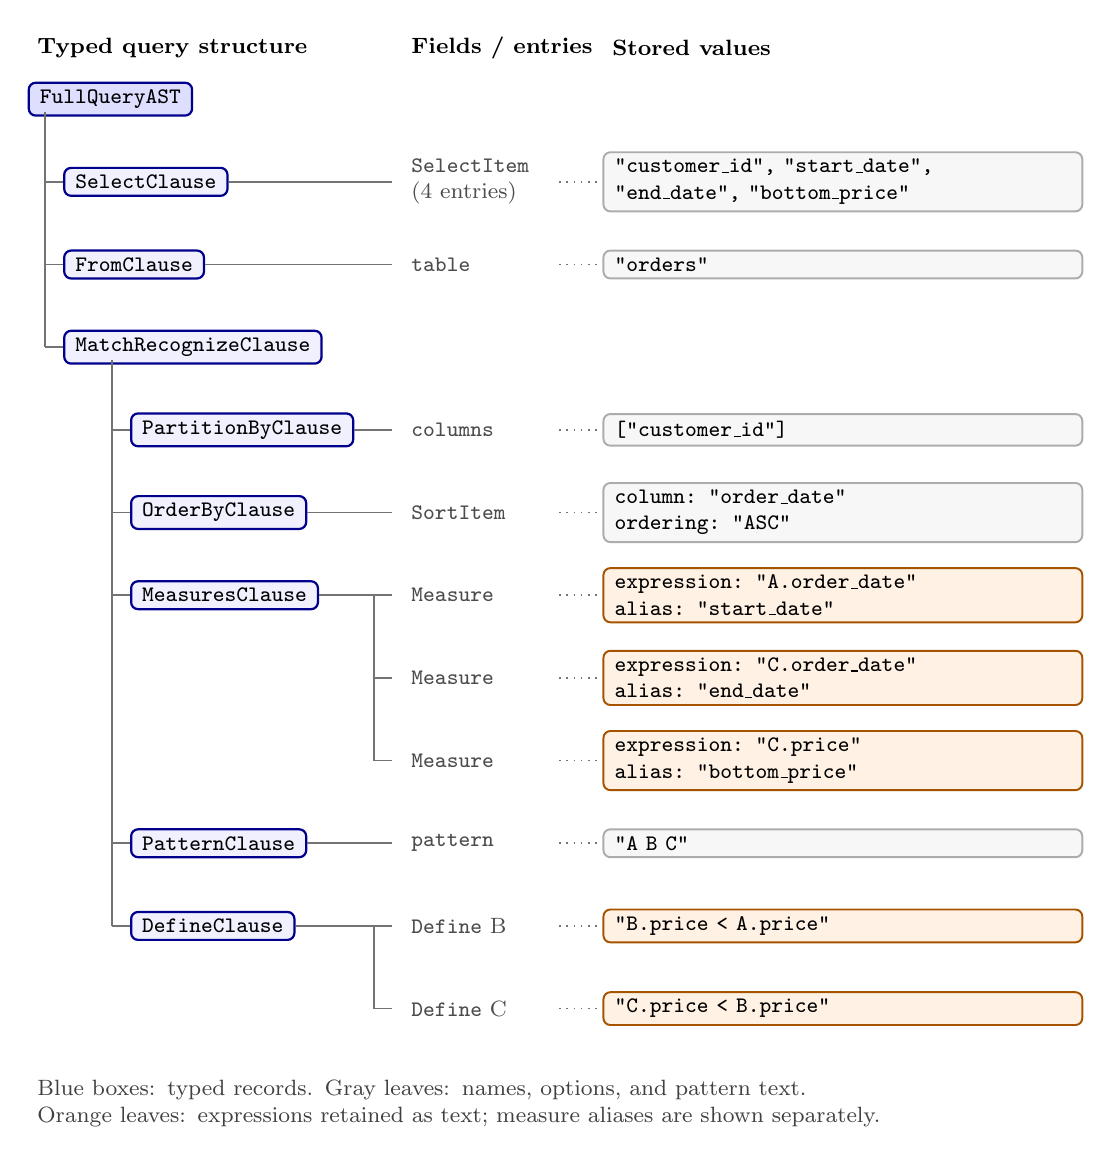
\begin{tikzpicture}[
    astnode/.style={draw=blue!55!black, rounded corners=2.5pt,
                    line width=0.8pt, fill=blue!6, anchor=west,
                    inner xsep=4pt, inner ysep=2.6pt,
                    font=\footnotesize\ttfamily},
    astroot/.style={astnode, fill=blue!13},
    astfield/.style={anchor=west, align=left,
                     font=\footnotesize, text=black!70},
    astleaf/.style={draw=gray!65, rounded corners=2.5pt,
                    line width=0.7pt, fill=gray!6, anchor=west,
                    align=left, text width=5.8cm,
                    inner xsep=4pt, inner ysep=2.6pt,
                    font=\footnotesize\ttfamily},
    astexpression/.style={astleaf, draw=orange!65!black,
                          fill=orange!10},
    spine/.style={draw=black!55, line width=0.6pt}
  ]
    \def\ra{-1.05} \def\cf{4.75} \def\cl{7.30}

    \node[anchor=west, font=\footnotesize\bfseries]
      at (0,0.65) {Typed query structure};
    \node[anchor=west, font=\footnotesize\bfseries]
      at (\cf,0.65) {Fields / entries};
    \node[anchor=west, font=\footnotesize\bfseries]
      at (\cl,0.65) {Stored values};

    \node[astroot]  (root) at (0,0)            {FullQueryAST};
    \node[astnode]  (sel)  at (0.45,1*\ra)     {SelectClause};
    \node[astnode]  (frm)  at (0.45,2*\ra)     {FromClause};
    \node[astnode]  (mrc)  at (0.45,3*\ra)     {MatchRecognizeClause};
    \node[astnode]  (prt)  at (1.30,4*\ra)     {PartitionByClause};
    \node[astnode]  (ord)  at (1.30,5*\ra)     {OrderByClause};
    \node[astnode]  (mea)  at (1.30,6*\ra)     {MeasuresClause};
    \node[astnode]  (pat)  at (1.30,9*\ra)     {PatternClause};
    \node[astnode]  (def)  at (1.30,10*\ra)    {DefineClause};

    \node[astfield] at (\cf,1*\ra)  {\texttt{SelectItem}\\(4 entries)};
    \node[astfield] at (\cf,2*\ra)  {\texttt{table}};
    \node[astfield] at (\cf,4*\ra)  {\texttt{columns}};
    \node[astfield] at (\cf,5*\ra)  {\texttt{SortItem}};
    \node[astfield] at (\cf,6*\ra)  {\texttt{Measure}};
    \node[astfield] at (\cf,7*\ra)  {\texttt{Measure}};
    \node[astfield] at (\cf,8*\ra)  {\texttt{Measure}};
    \node[astfield] at (\cf,9*\ra)  {\texttt{pattern}};
    \node[astfield] at (\cf,10*\ra) {\texttt{Define} B};
    \node[astfield] at (\cf,11*\ra) {\texttt{Define} C};

    \node[astleaf] at (\cl,1*\ra)
      {"customer\_id", "start\_date",\\"end\_date", "bottom\_price"};
    \node[astleaf] at (\cl,2*\ra)  {"orders"};
    \node[astleaf] at (\cl,4*\ra)  {["customer\_id"]};
    \node[astleaf] at (\cl,5*\ra)
      {column: "order\_date"\\ordering: "ASC"};
    \node[astexpression] at (\cl,6*\ra)
      {expression: "A.order\_date"\\alias: "start\_date"};
    \node[astexpression] at (\cl,7*\ra)
      {expression: "C.order\_date"\\alias: "end\_date"};
    \node[astexpression] at (\cl,8*\ra)
      {expression: "C.price"\\alias: "bottom\_price"};
    \node[astleaf] at (\cl,9*\ra)  {"A B C"};
    \node[astexpression] at (\cl,10*\ra) {"B.price < A.price"};
    \node[astexpression] at (\cl,11*\ra) {"C.price < B.price"};

    \draw[spine] (0.22,-0.16) -- (0.22,3*\ra) ;
    \foreach \y in {1,2,3} \draw[spine] (0.22,\y*\ra) -- (0.45,\y*\ra);
    \draw[spine] (1.07,3*\ra-0.16) -- (1.07,10*\ra);
    \foreach \y in {4,5,6,9,10} \draw[spine] (1.07,\y*\ra) -- (1.30,\y*\ra);
    \foreach \y in {1,2,4,5,6,7,8,9,10,11}
      \draw[spine, dotted] (\cf+2.0,\y*\ra) -- (\cl-0.06,\y*\ra);
    \draw[spine] (mea.east) -- (\cf-0.35,6*\ra);
    \draw[spine] (\cf-0.35,6*\ra) -- (\cf-0.35,8*\ra);
    \foreach \y in {6,7,8} \draw[spine] (\cf-0.35,\y*\ra) -- (\cf-0.12,\y*\ra);
    \draw[spine] (def.east) -- (\cf-0.35,10*\ra);
    \draw[spine] (\cf-0.35,10*\ra) -- (\cf-0.35,11*\ra);
    \foreach \y in {10,11} \draw[spine] (\cf-0.35,\y*\ra) -- (\cf-0.12,\y*\ra);
    \draw[spine] (sel.east) -- (\cf-0.12,1*\ra);
    \draw[spine] (frm.east) -- (\cf-0.12,2*\ra);
    \draw[spine] (prt.east) -- (\cf-0.12,4*\ra);
    \draw[spine] (ord.east) -- (\cf-0.12,5*\ra);
    \draw[spine] (pat.east) -- (\cf-0.12,9*\ra);

    \node[anchor=north west, align=left, text width=13.1cm,
          font=\footnotesize, text=black!75]
      at (0,11.75*\ra)
      {Blue boxes: typed records.  Gray leaves: names, options, and pattern text.\\
       Orange leaves: expressions retained as text; measure aliases are shown separately.};
  \end{tikzpicture}
  \caption[Typed AST for the worked orders query]{Typed AST for the
    worked \texttt{orders} query in Figure~\ref{fig:orders-pipeline}.
    The tree separates the outer query from its row-pattern clause.
    Expression strings remain unexpanded.  Metadata and absent optional
    clauses are omitted.}
  \label{fig:meth-ast}
\end{figure}

\paragraph{Safe expression evaluation.}
These predicate and measure strings come from the user, so the engine
never runs them as Python code.  It reads each one into a small tree of operations and
walks that tree itself.  This is the \emph{Interpreter} pattern: a
parser turns the text into a tree, and an evaluator walks that tree,
interprets each node, and returns a value.  The walk uses an
\emph{allowlist}: an operation is evaluated only when the engine has a
handler for it.  Safety therefore comes from the allowlist itself, not
from blocking unsafe cases one at a time.

The allowlist includes comparisons, Boolean and arithmetic operators,
literals, \texttt{IN} lists, conditional expressions, qualified
references such as \texttt{A.price}, navigation functions,
\texttt{CLASSIFIER}, \texttt{MATCH\_NUMBER}, and the supported
aggregates.  Everything else falls outside it: imports, assignments,
and access to Python built-ins are never evaluated.  An expression sees
only its explicit evaluation context: ordered rows, pattern bindings,
and match metadata.

The front end is exercised by dedicated tests.  They include
adversarial inputs such as undefined variables, prohibited function
forms, invalid skip targets, and incompatible output-mode
combinations.  They also include end-to-end scenarios adapted from
Trino's row-pattern tests.

\paragraph{Outside this path.}
General subquery planning and SQL features outside the supported
row-pattern subset are not handled here.  Vendor extensions may also
need parser and evaluator changes.

% ----------------------------------------------------------------
\section{Semantic Validation}
\label{sec:meth-semantic}
% ----------------------------------------------------------------

Parsing proves that a query is well formed, but not that it is
semantically valid.  For example, \texttt{PATTERN (A B)} with
\texttt{DEFINE B AS B.price > Q.price} parses correctly, but
\texttt{Q} is not declared by the pattern.

A validation pass runs while the AST is completed and before any
automaton is built.  It rejects invalid references and unsupported
clause combinations.  The next stage then supplies defaults and builds
the execution configuration.  At this point no input row has been
matched, so errors can still identify the clause that caused them.

\emph{Every reference must resolve.}  This is ordinary \emph{name
resolution}, with the pattern as its scope.  For ordinary patterns, the
front end checks qualified references in \texttt{DEFINE} and
\texttt{MEASURES} against the pattern variables and \texttt{SUBSET}
aliases.  Specialized \texttt{PERMUTE} validation continues during
pattern handling.  A subset such as \texttt{SUBSET U = (A, B)} lets
\texttt{U.price} refer to rows matched by either member.  A variable
without \texttt{DEFINE} is valid because its predicate is implicitly
true.  DataFrame column names are resolved later, when the execution
configuration is applied to the input.

\emph{Calls must use a supported form.}  The front end checks the
syntax of navigation functions and selected aggregates.  Detailed
aggregate argument checks also run before an aggregate is evaluated.
For example, \texttt{COUNT\_IF} takes one condition, while
\texttt{SUM\_IF} and \texttt{AVG\_IF} take a value and a condition.
This validation does not try to prove that a predicate can become true;
a valid predicate may simply produce no match.

\emph{Settings must work together.}  Some combinations ask for
contradictory output.  An exclusion, written \texttt{\{-\ \ldots\ -\}},
keeps matched rows out of the result, while the
\texttt{WITH UNMATCHED ROWS} form of \texttt{ALL ROWS PER MATCH} asks
for every row to appear.  One removes what the other requires, so the
standard forbids the pair.  The validator therefore rejects it.  An
\texttt{AFTER MATCH SKIP} target must also name a pattern variable or
subset.  Whether the target occurs in a particular match is known only
at runtime.  The matcher therefore rejects an absent target or a skip
position that would make no progress.  The output mode, skip mode,
implicit predicates, and measure modes then pass to logical-plan
construction (Section~\ref{sec:meth-logical}).

% ................................................................
\section{Logical Plan Construction}
\label{sec:meth-logical}
% ................................................................

The logical plan is a resolved execution configuration.  It collects
the typed AST fields pulled from the \texttt{MatchRecognizeClause} that compilation and matching need
(Table~\ref{tab:logical-plan}).  Later stages do not reparse the full
SQL query.  Pattern, predicate, and measure text remain available to
their dedicated compilers and evaluators.

\begin{table}[htbp]
  \centering
  \caption{Principal fields in the logical execution configuration}
  \label{tab:logical-plan}
  \small
  \setlength{\tabcolsep}{4pt}
  \begin{tabular}{llp{6.2cm}}
    \toprule
    \textbf{Attribute} & \textbf{Type} & \textbf{Semantics} \\
    \midrule
    \texttt{partition\_by}   & \texttt{List[str]}
      & Columns for DataFrame partitioning; empty means a single
        global partition \\[4pt]
    \texttt{order\_by}       & \texttt{List[str]}
      & Direct columns used for intra-partition ordering \\[4pt]
    \texttt{order\_ascending} & \texttt{List[bool]}
      & Per-key ascending or descending direction \\[4pt]
    \texttt{order\_nulls}   & \texttt{List[str]}
      & Per-key null placement; omitted placement defaults to
        \texttt{NULLS LAST} \\[4pt]
    \texttt{pattern\_text}   & \texttt{str}
      & Normalized pattern string forwarded to the tokenizer \\[4pt]
    \texttt{define}          & \texttt{Dict[str, str]}
      & Explicit variable $\to$ predicate mappings; absent mappings are
        treated as implicit true during matching \\[4pt]
    \texttt{subset\_dict}    & \texttt{Dict[str, List[str]]}
      & Subset alias $\to$ constituent variables \\[4pt]
    \texttt{measures}        & \texttt{Dict[str, str]}
      & Measure alias $\to$ expression string \\[4pt]
    \texttt{measure\_semantics} & \texttt{Dict[str, str]}
      & Measure alias $\to$ \texttt{"RUNNING"}/\texttt{"FINAL"}, per
        the rules in Figure~\ref{fig:measure-sem-resolution} \\[4pt]
    \texttt{rows\_per\_match} & \texttt{RowsPerMatch}
      & Output-row multiplicity \\[4pt]
    \texttt{skip\_mode}      & \texttt{SkipMode}
      & After-match skip strategy \\[4pt]
    \texttt{skip\_var}       & \texttt{Optional[str]}
      & Target variable/alias for \textsc{To First}/\textsc{To Last} \\
    \bottomrule
  \end{tabular}
\end{table}

Two defaults matter.  A variable without \texttt{DEFINE} uses an
implicit true predicate.  Measure semantics follow the priority rules
in Figure~\ref{fig:measure-sem-resolution}.  An explicit
\texttt{RUNNING} or \texttt{FINAL} prefix wins.
\texttt{ONE ROW PER MATCH} uses final values.  Under
\texttt{ALL ROWS PER MATCH}, navigation rules are resolved before
aggregate defaults.  \textsc{Running} sees rows through the current
output row; \textsc{Final} sees the complete match.

\begin{figure}[H]
  \centering
  \begin{tikzpicture}[
    node distance=0.30cm and 0.62cm,
    font=\footnotesize,
    msscan/.style={draw=black!65, rounded corners=2pt, thick,
                   fill=black!8, text width=9.4cm, minimum height=0.62cm,
                   align=center, inner sep=4pt},
    msstart/.style={draw=black!65, rounded corners=2pt, thick,
                    fill=blue!9, text width=7.5cm, minimum height=0.56cm,
                    align=center, inner sep=3pt},
    mstest/.style={draw=black!65, rounded corners=2pt, thick,
                   fill=white, text width=7.5cm, minimum height=0.48cm,
                   align=center, inner sep=3pt},
    msdeclared/.style={draw=black!70, rounded corners=2pt, thick, dashed,
                       fill=black!4, text width=2.05cm, minimum height=0.44cm,
                       align=center, inner sep=3pt},
    msfinal/.style={draw=black!75, double, rounded corners=2pt, thick,
                    fill=green!9, text width=2.05cm, minimum height=0.44cm,
                    align=center, inner sep=3pt},
    msrunning/.style={draw=black!75, rounded corners=2pt, very thick,
                      fill=blue!13, text width=2.05cm, minimum height=0.44cm,
                      align=center, inner sep=3pt},
    msnote/.style={draw=black!45, rounded corners=2pt,
                   fill=black!3, text width=11.8cm,
                   align=left, inner sep=4pt, font=\scriptsize},
    arrow/.style={-{Stealth[length=1.9mm]}, thick, black!75},
    yes/.style={font=\scriptsize, above, inner sep=2pt},
    no/.style={font=\scriptsize, right, inner sep=2pt}
  ]
    \node[msscan] (scan)
      {\textbf{Query pre-scan (once)}\\[-2pt]
       Set $E=\mathrm{true}$ when any measure has an explicit leading\\[-2pt]
       \texttt{RUNNING} or \texttt{FINAL} prefix.};
    \node[msstart, below=of scan] (current)
      {\textbf{For each measure $m$}\\[-2pt]
       Apply the first matching rule.};

    \node[mstest, below=of current] (explicit)
      {1.\ Does $m$ have an explicit \texttt{RUNNING} or \texttt{FINAL} prefix?};
    \node[msdeclared, right=of explicit] (stated)
      {use declared mode};

    \node[mstest, below=of explicit] (one)
      {2.\ Does the query return one row per match?};
    \node[msfinal, right=of one] (onefinal) {\textsc{Final}};

    \node[mstest, below=of one] (leadnav)
      {3.\ Does it \emph{start with} \texttt{FIRST}, \texttt{PREV}, or \texttt{NEXT}?};
    \node[msfinal, right=of leadnav] (leadfinal) {\textsc{Final}};

    \node[mstest, below=of leadnav] (leadlast)
      {4.\ Does it \emph{start with} \texttt{LAST}?};
    \node[msrunning, left=of leadlast] (leadrun) {\textsc{Running}};

    \node[mstest, below=of leadlast] (hasnav)
      {5.\ Does it use \texttt{FIRST}, \texttt{PREV}, or \texttt{NEXT} anywhere?};
    \node[msfinal, right=of hasnav] (navfinal) {\textsc{Final}};

    \node[mstest, below=of hasnav] (haslast)
      {6.\ Does it use \texttt{LAST} anywhere?};
    \node[msrunning, left=of haslast] (lastrun) {\textsc{Running}};

    \node[mstest, below=of haslast] (mixed)
      {7.\ Is $E=\mathrm{true}$?};
    \node[msfinal, right=of mixed] (mixedfinal) {\textsc{Final}};

    \node[mstest, below=of mixed] (aggregate)
      {8.\ Does it start with a default-running aggregate?\textsuperscript{*}};
    \node[msrunning, left=of aggregate] (aggrun) {\textsc{Running}};

    \node[msfinal, below=of aggregate, text width=7.5cm] (fallback)
      {9.\ Otherwise: \textsc{Final}};

    \node[msnote, below=0.42cm of fallback] (aggregatekey)
      {\textsuperscript{*}\textbf{Default-running aggregates:}
       \texttt{COUNT}, \texttt{SUM}, \texttt{ARRAY\_AGG},
       \texttt{MAX\_BY}, \texttt{MIN\_BY}, \texttt{STRING\_AGG},
       \texttt{COUNT\_IF}, \texttt{SUM\_IF}, and \texttt{AVG\_IF}.};
    \node[msnote, below=0.20cm of aggregatekey] (meaning)
      {\textbf{Meaning:} \textsc{Running} uses rows through the current
       output row; \textsc{Final} uses the complete match.};

    \draw[arrow] (scan) -- (current);
    \draw[arrow] (current) -- (explicit);
    \foreach \a/\b in {explicit/stated, one/onefinal, leadnav/leadfinal,
                       hasnav/navfinal, mixed/mixedfinal}
      \draw[arrow] (\a) -- node[yes]{yes} (\b);
    \foreach \a/\b in {leadlast/leadrun, haslast/lastrun,
                       aggregate/aggrun}
      \draw[arrow] (\a) -- node[yes]{yes} (\b);
    \foreach \a/\b in {explicit/one, one/leadnav, leadnav/leadlast,
                       leadlast/hasnav, hasnav/haslast, haslast/mixed,
                       mixed/aggregate, aggregate/fallback}
      \draw[arrow] (\a) -- node[no]{no} (\b);
  \end{tikzpicture}
  \caption{Resolving \texttt{RUNNING} and \texttt{FINAL} semantics.}
  \label{fig:measure-sem-resolution}
\end{figure}

With these attributes resolved, the execution configuration is handed
to the pattern-compilation phase of Chapter~\ref{chap:implementation}.

% ----------------------------------------------------------------
\section{Chapter Summary}
\label{sec:meth-summary}
% ----------------------------------------------------------------

This chapter presented the five-stage design and its front-end
boundaries.  Parsing and validation create a checked AST.  Logical-plan
construction resolves the execution configuration, including output,
skip, and measure modes.  The design reuses the Trino ANTLR4 grammar
and evaluates user expressions through a restricted AST evaluator.
Chapter~\ref{chap:implementation} continues with automata compilation,
Pandas execution, and optimization.
